%% -------------------------------------------------------------------------------------
% This is a general template file for preparing an article for Revista Colombiana de Estad�stica
% *************************************************************************************
\documentclass[english]{revcoles}
\usepackage[top=3cm,,bottom=3cm]{geometry}
\usepackage[latin1]{inputenc}
\usepackage{graphicx}
%
\hyphenation{}
% //// --------------------------------------------------------------------------------
\begin{document}

\title[maintitle = Gr\'{a}ficos de Control Multivariantes,
]

\begin{authors}
\author[firstname = Kevin,
        surname = Garc�a,
        numberinstitution = 1,
        code= 1533173,
        affiliation = Universidad del Valle,
        email = kevin.chica@correounivalle.edu.co]
\author[firstname = Alejandro,
        surname = Vargas,
        numberinstitution = 1,
        code= 1525953,
        affiliation = Universidad del Valle,
        email = jose.alejandro.vargas@correounivalle.edu.co]
\end{authors}
%
\begin{institutions}
     \institute[subdivision = Departamento de estad�stica,
                institution = Universidad del Valle,
                city = Cali,
                country = Colombia]
\end{institutions}

\begin{secondaryabstract}
Los m�todos de muestreo tipo aceptaci�n y rechazo juegan un papel sumamente importante en el �rea de control de calidad, de aqu� que d�a a d�a se desarrollen nuevas t�cnicas que optimicen los procesos de calidad. En el siguiente art�culo se ver�n replicadas las propuestas de Squeglia en cuanto a c�mo trabajar con un m�todo en el que se impone como requisito de aceptaci�n cero defectuosos en la muestra. Se realizaron comparaciones entre los m�todos tradicionalmente utilizados, con el m�todo c=0; para estas comparaciones se utilizaron curvas caracter�sticas de operaciones, valores de AOQL, probabilidades de aceptaci�n, y todo esto en contraste con diferentes tama�os de muestra, donde observamos que el m�todo propuesto en comparaci�n con el m�todo MIL-STD-105E/ANSI Z1.4 protegen a�n m�s al consumidor, siendo este m�todo mas estricto  a la hora de aceptar lotes con cantidades ``grandes'' de defectuosos. El m�todo por otra parte ``castiga'' al productor, ya que si este no tiene una calidad cercana al 100\%, tiende a rechazar muchos m�s lotes.



\end{secondaryabstract}

\section{Introducci�n}


\section{Antecedentes}

\section{Descripci�n metodolog�a de aplicaci�n}

\section{Caso ilustrativo}

\section{Conclusiones}

    \bibliography{references}

\nocite{ControlR}
    \appendix% !don't modify this line�

\section{Curvas de operaci�n}
\begin{figure}[h!]
  \centering
  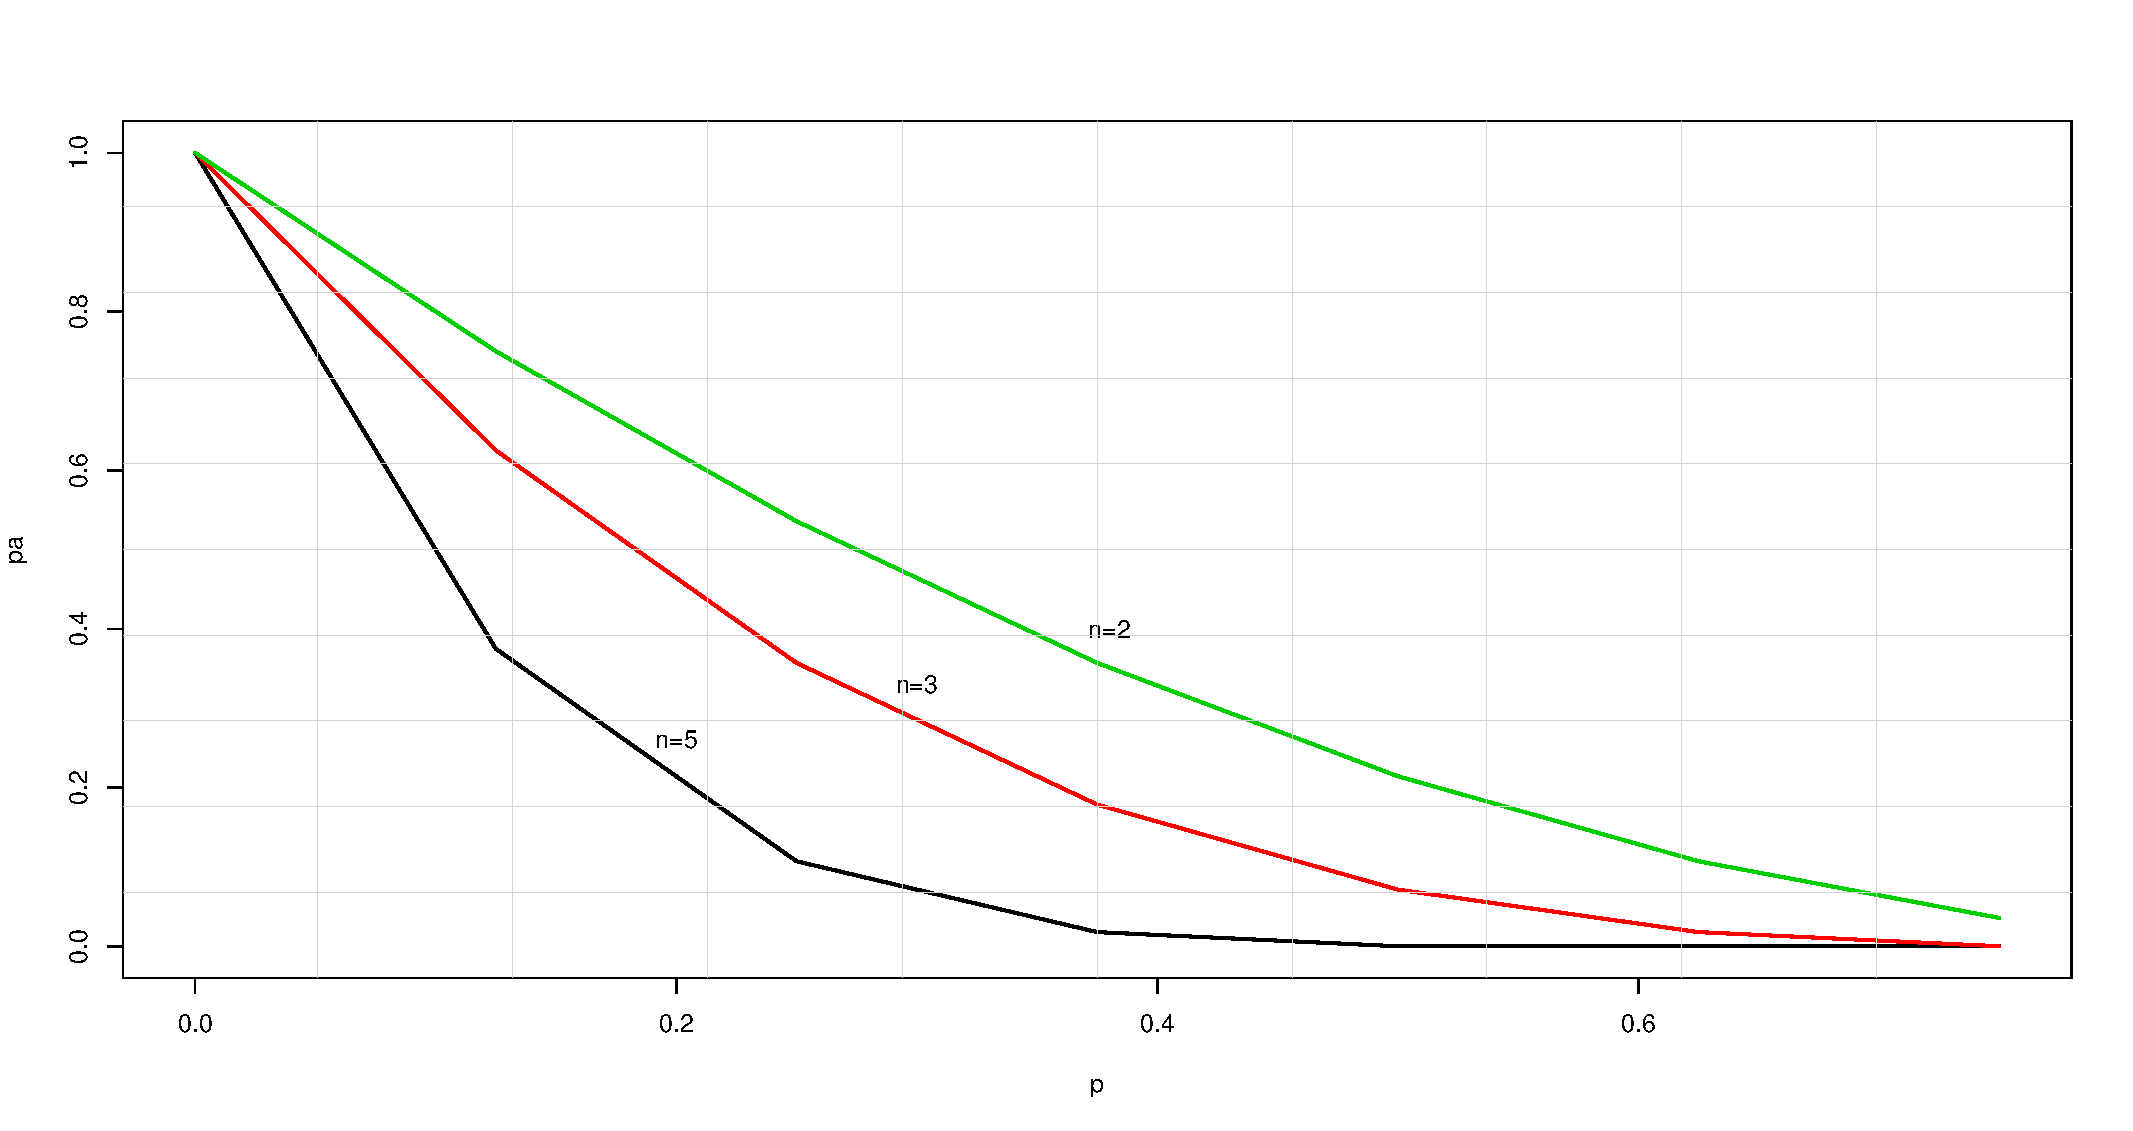
\includegraphics[scale=0.45]{FigurasUV/CO1.pdf}
  \caption{Curvas OC para planes de muestreo simples con C=0. Tama�o del lote 2 - 8}
\end{figure}



\end{document}

